



%\begin{figure}[!tbp]
%  \centering
%  \begin{minipage}[H]{0.4\textwidth}
%    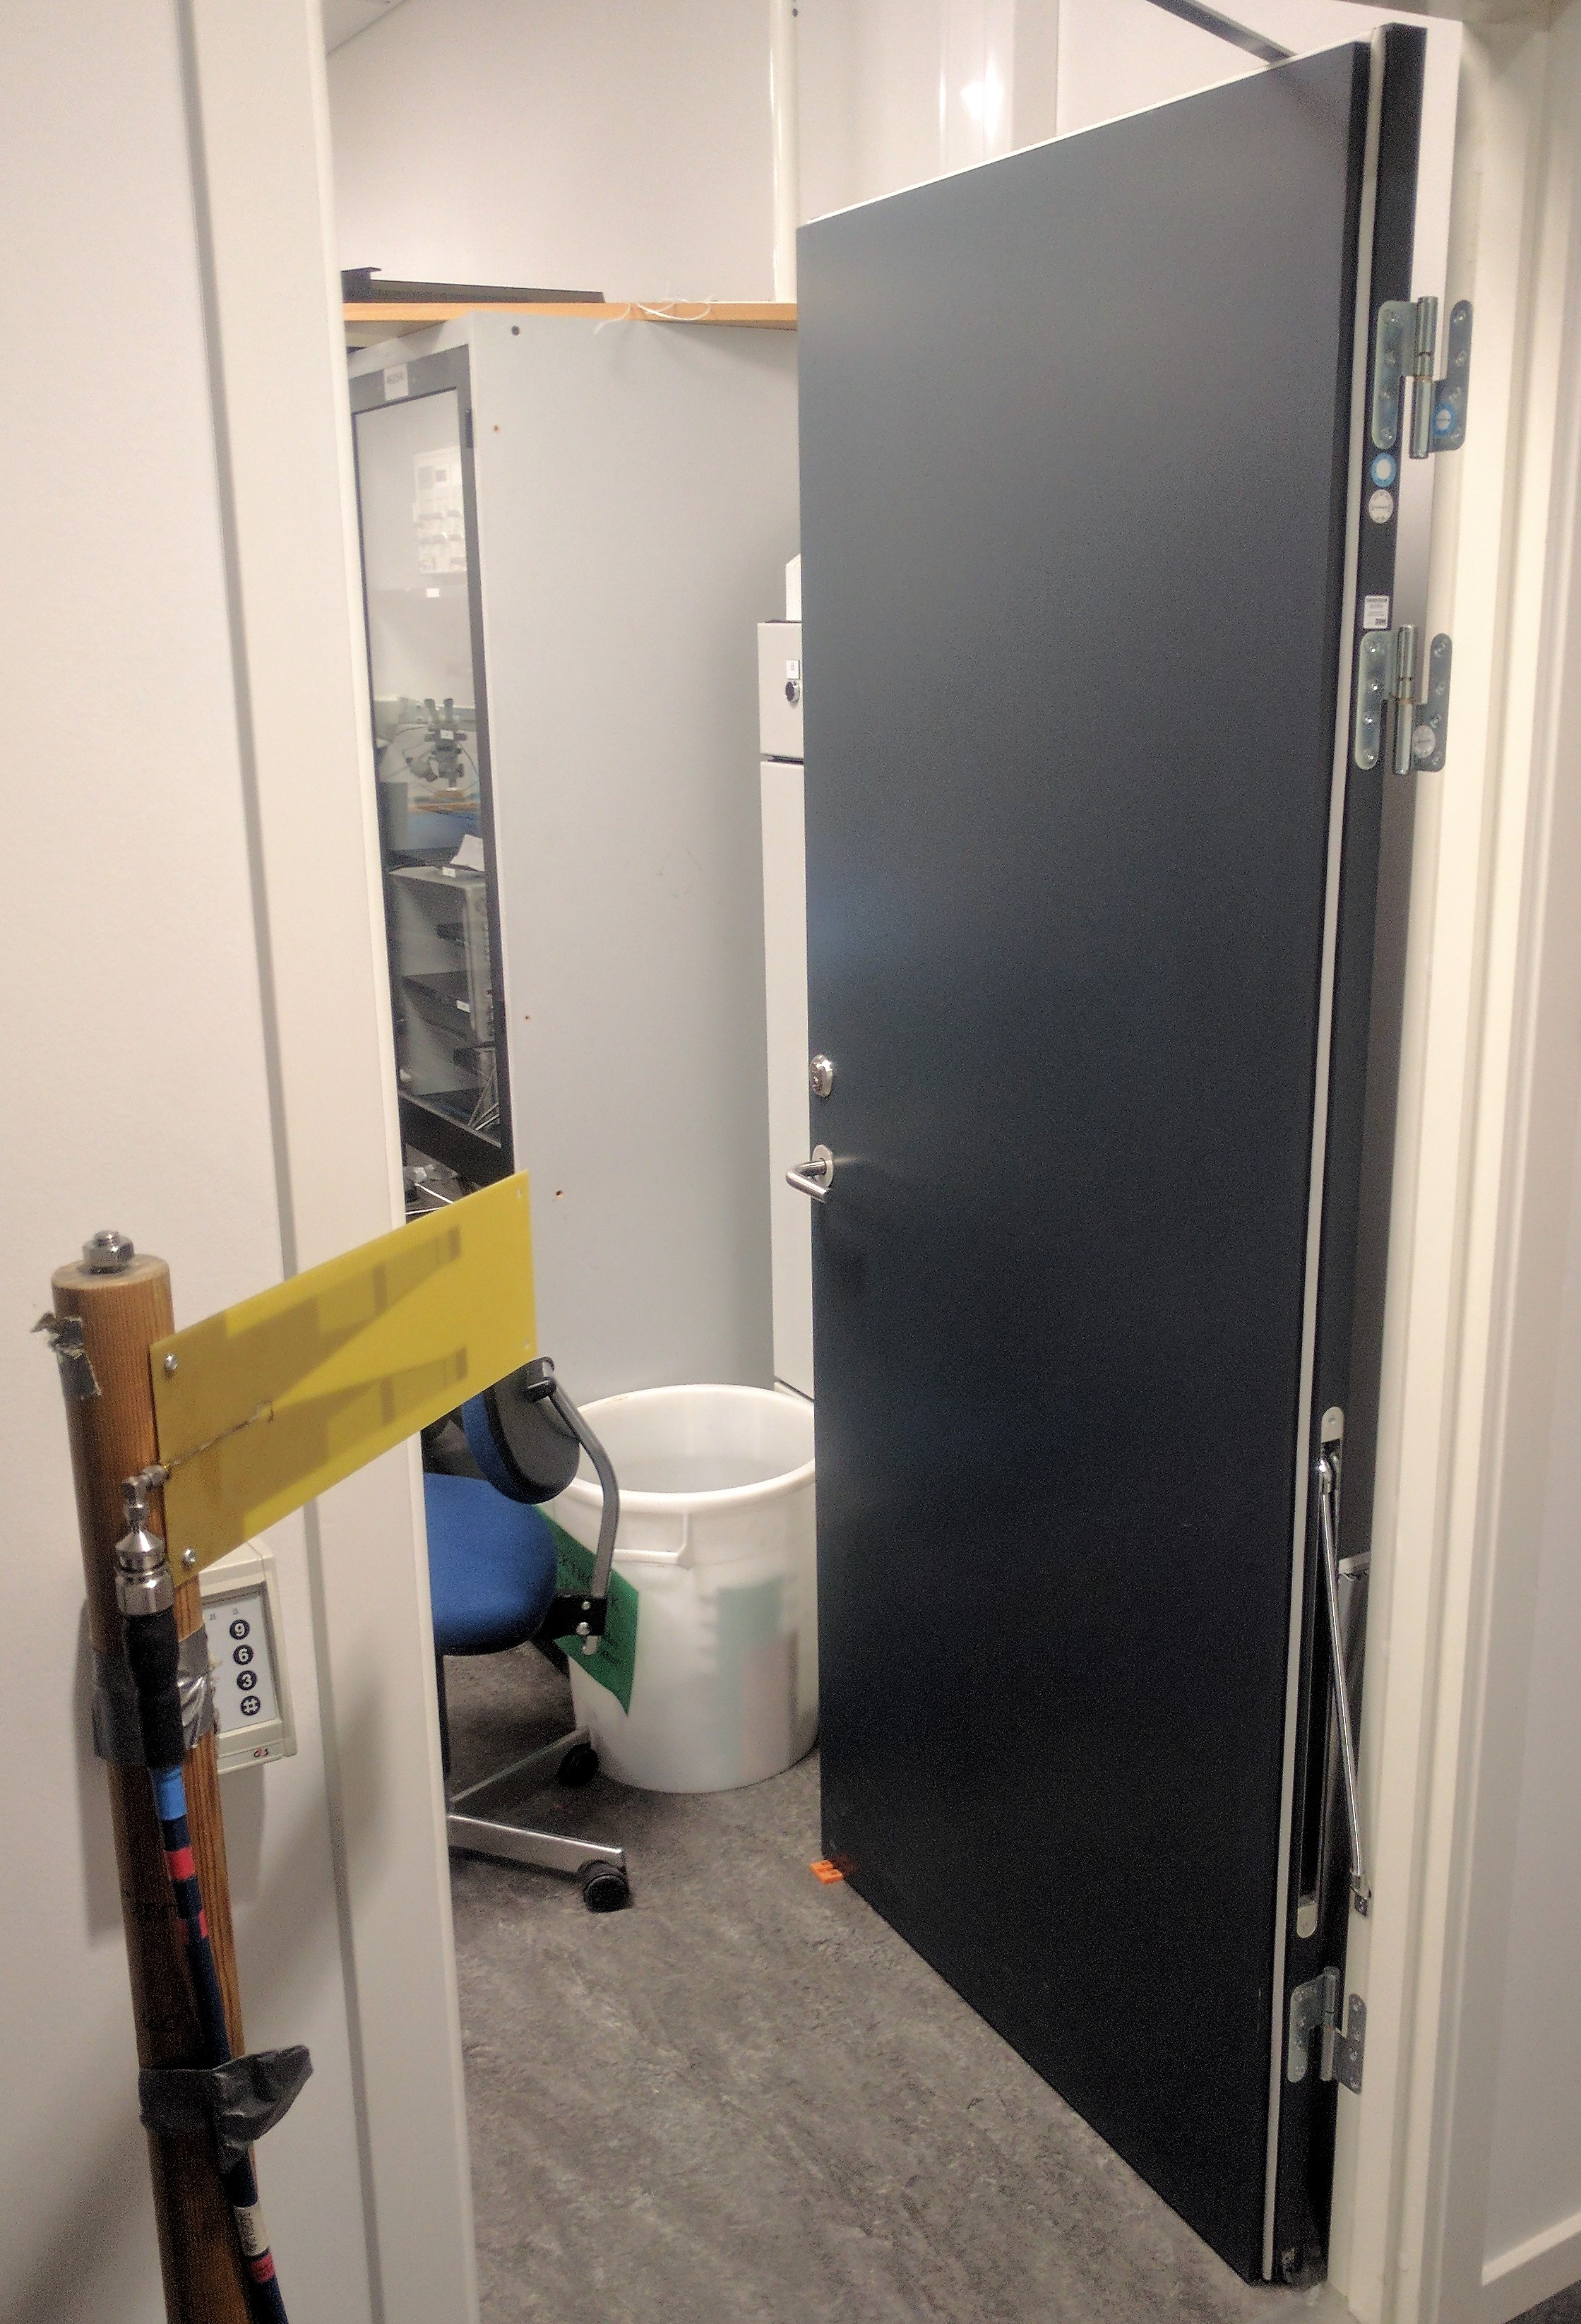
\includegraphics[width=\textwidth]{pictures/Measurement/antenna_door.jpg}
%    \caption{Directional TX antenna.}
%  \end{minipage}
%  \hfill
%  \begin{minipage}[H]{0.1\textwidth}
%    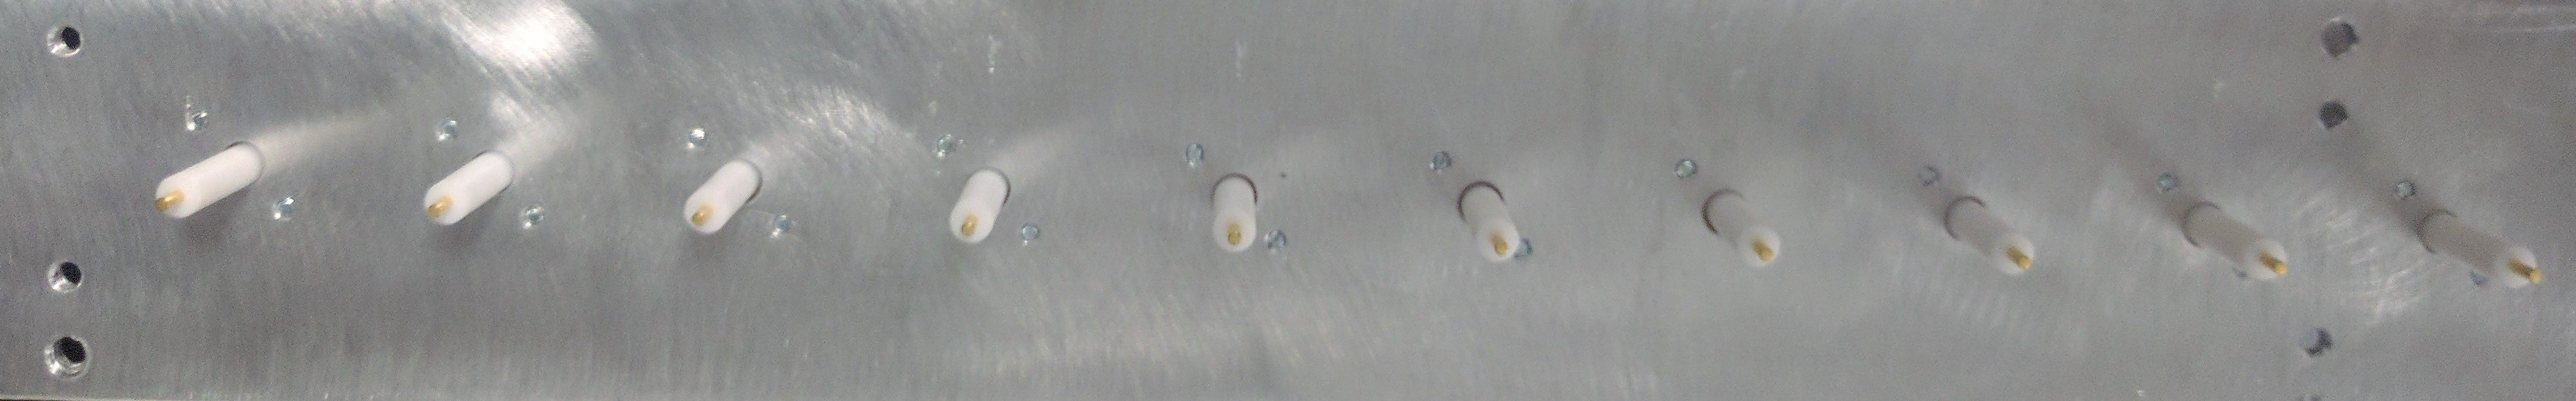
\includegraphics[width=\textwidth]{pictures/Measurement/antenna_array.jpg}
%    \caption{omnidirectional RX antenna array with $\frac{\lambda}{2}$ spacing}
%  \end{minipage}
%\end{figure}





\chapter{Available Resources}
\section{Environment}
The HF lab was the room used for the measurements, it has  clutter and surfaces to give  multipath propagation. The TX antenna is placed outside of the room pointing towards the door. This provides a NLOS condition. The RX antenna array is moved across the opposite side of the room.

\begin{figure}[H]
  \centering
  \begin{minipage}[H]{0.4\textwidth}
    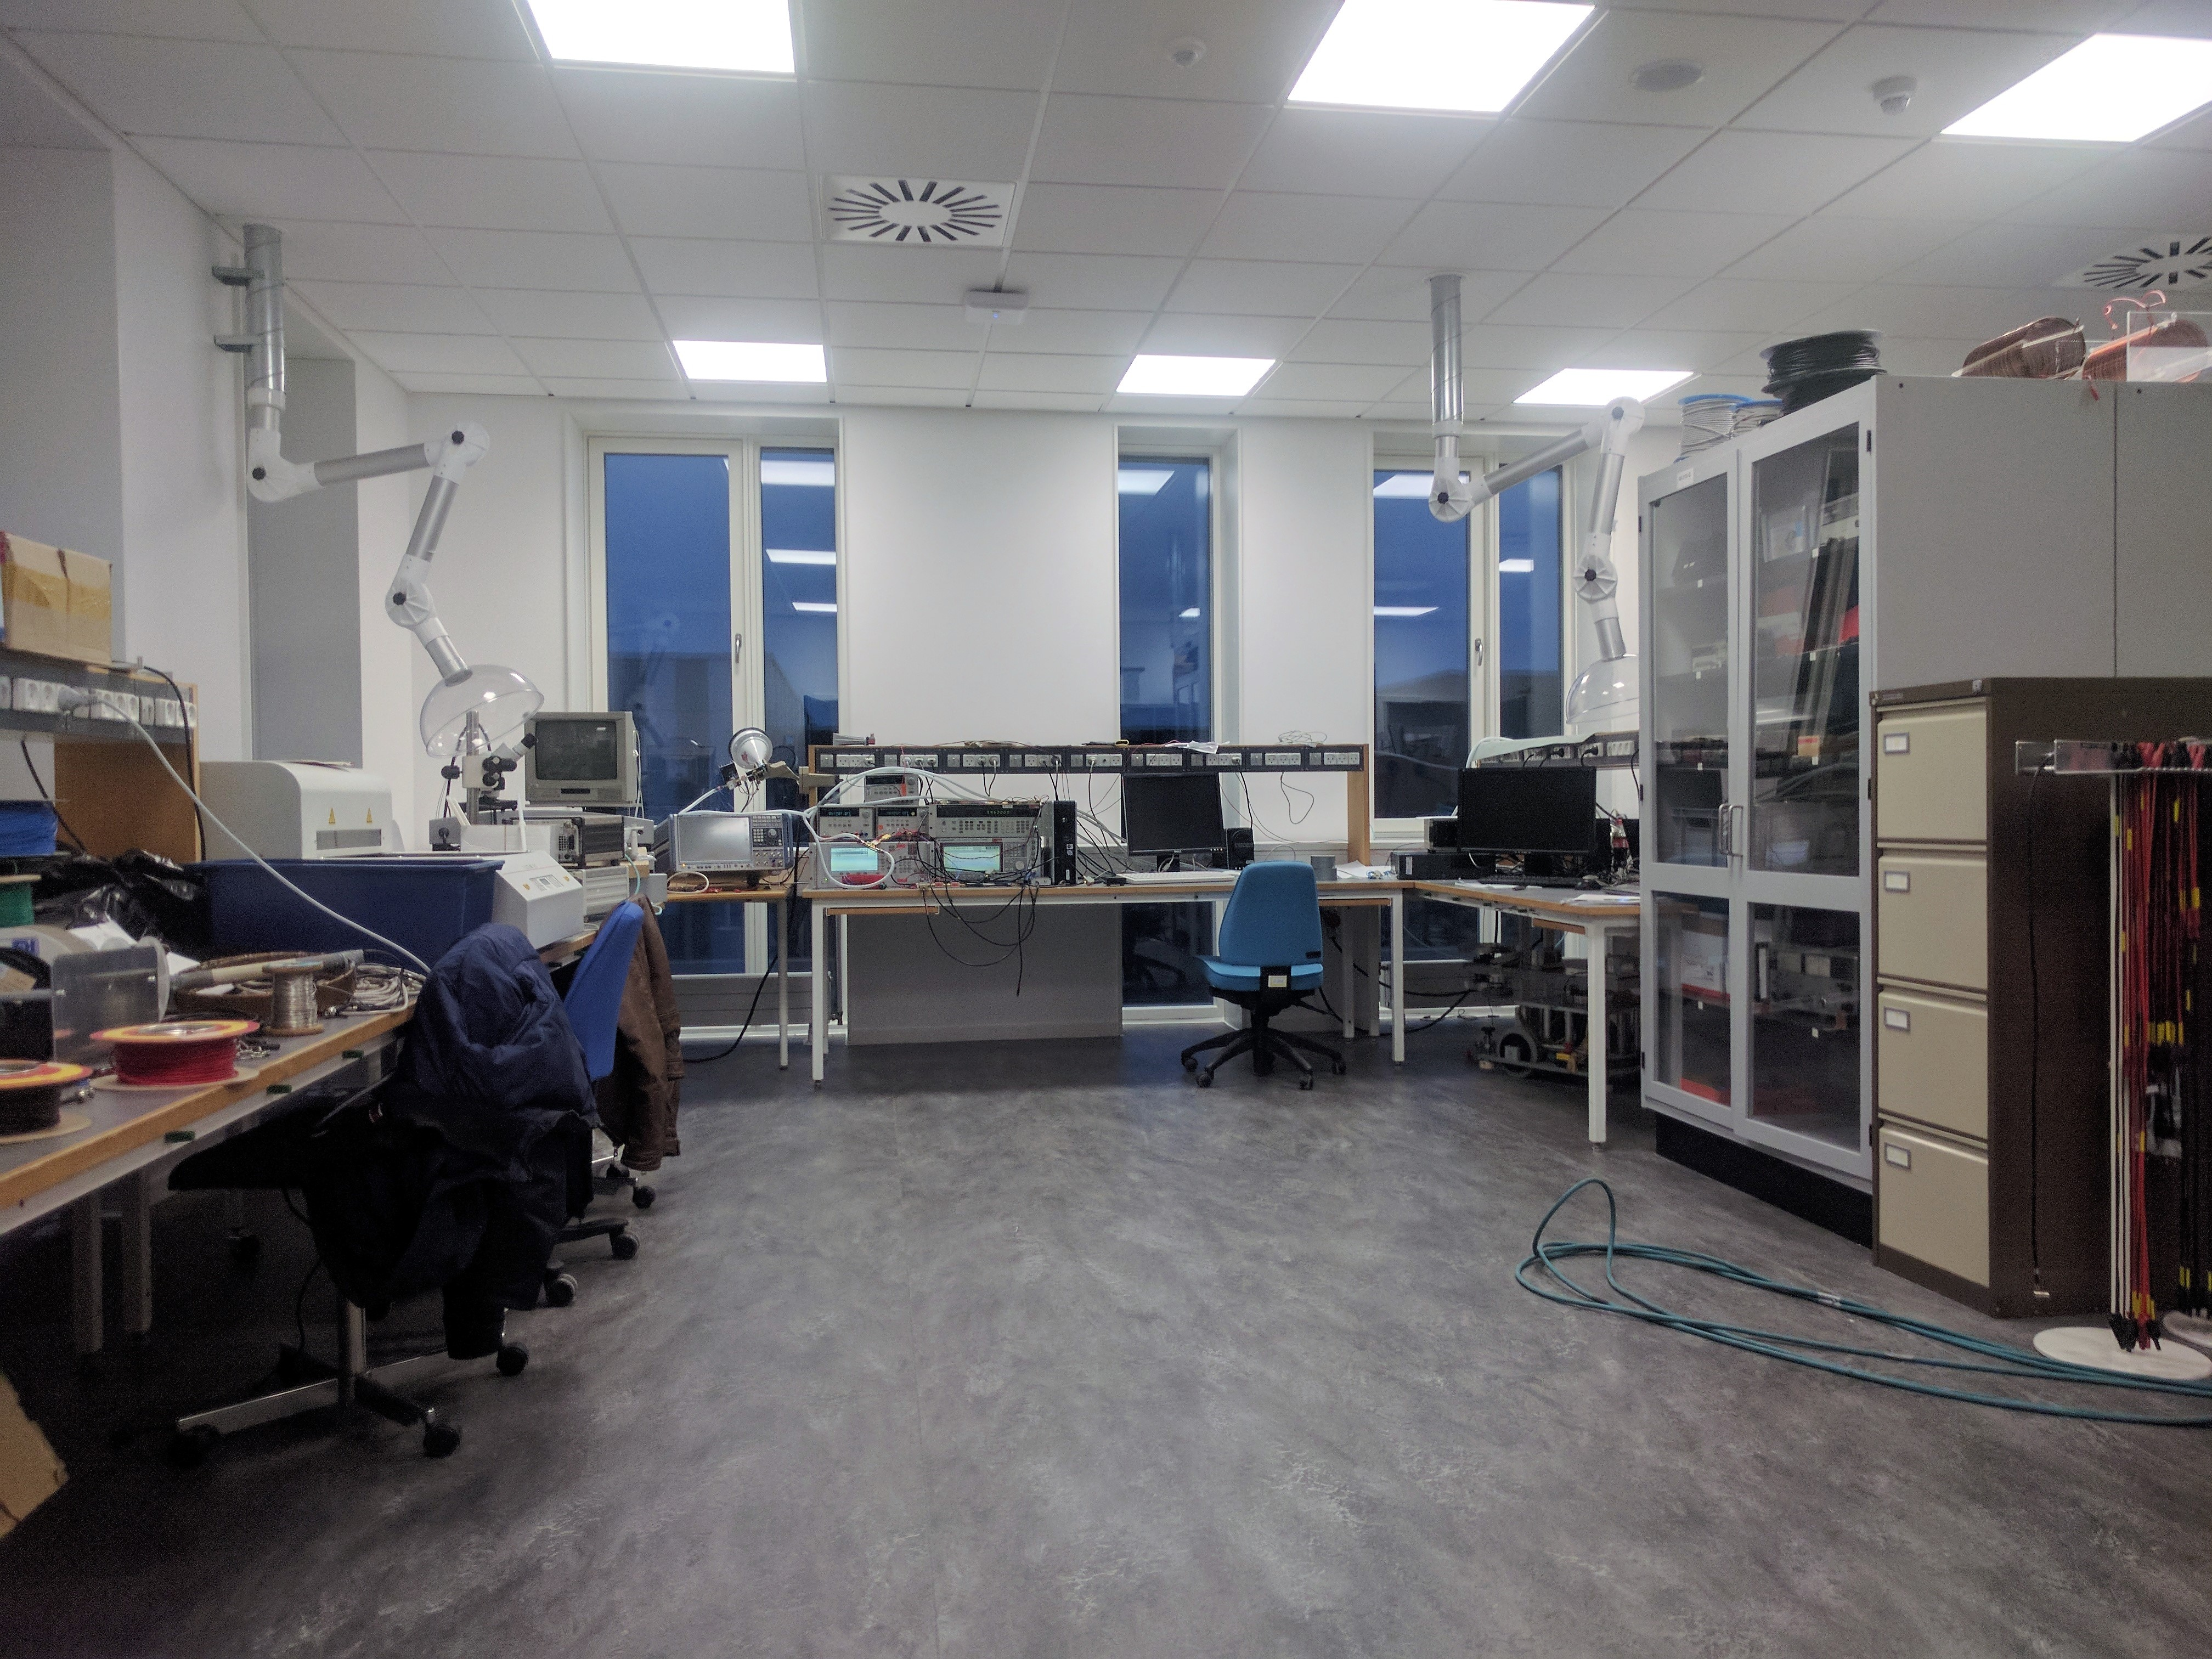
\includegraphics[width=\textwidth]{pictures/Measurement/walking_meas.jpg}
    \caption{Area of the fading gain measurements}
  \end{minipage}
  \hfill
  \begin{minipage}[H]{0.4\textwidth}
    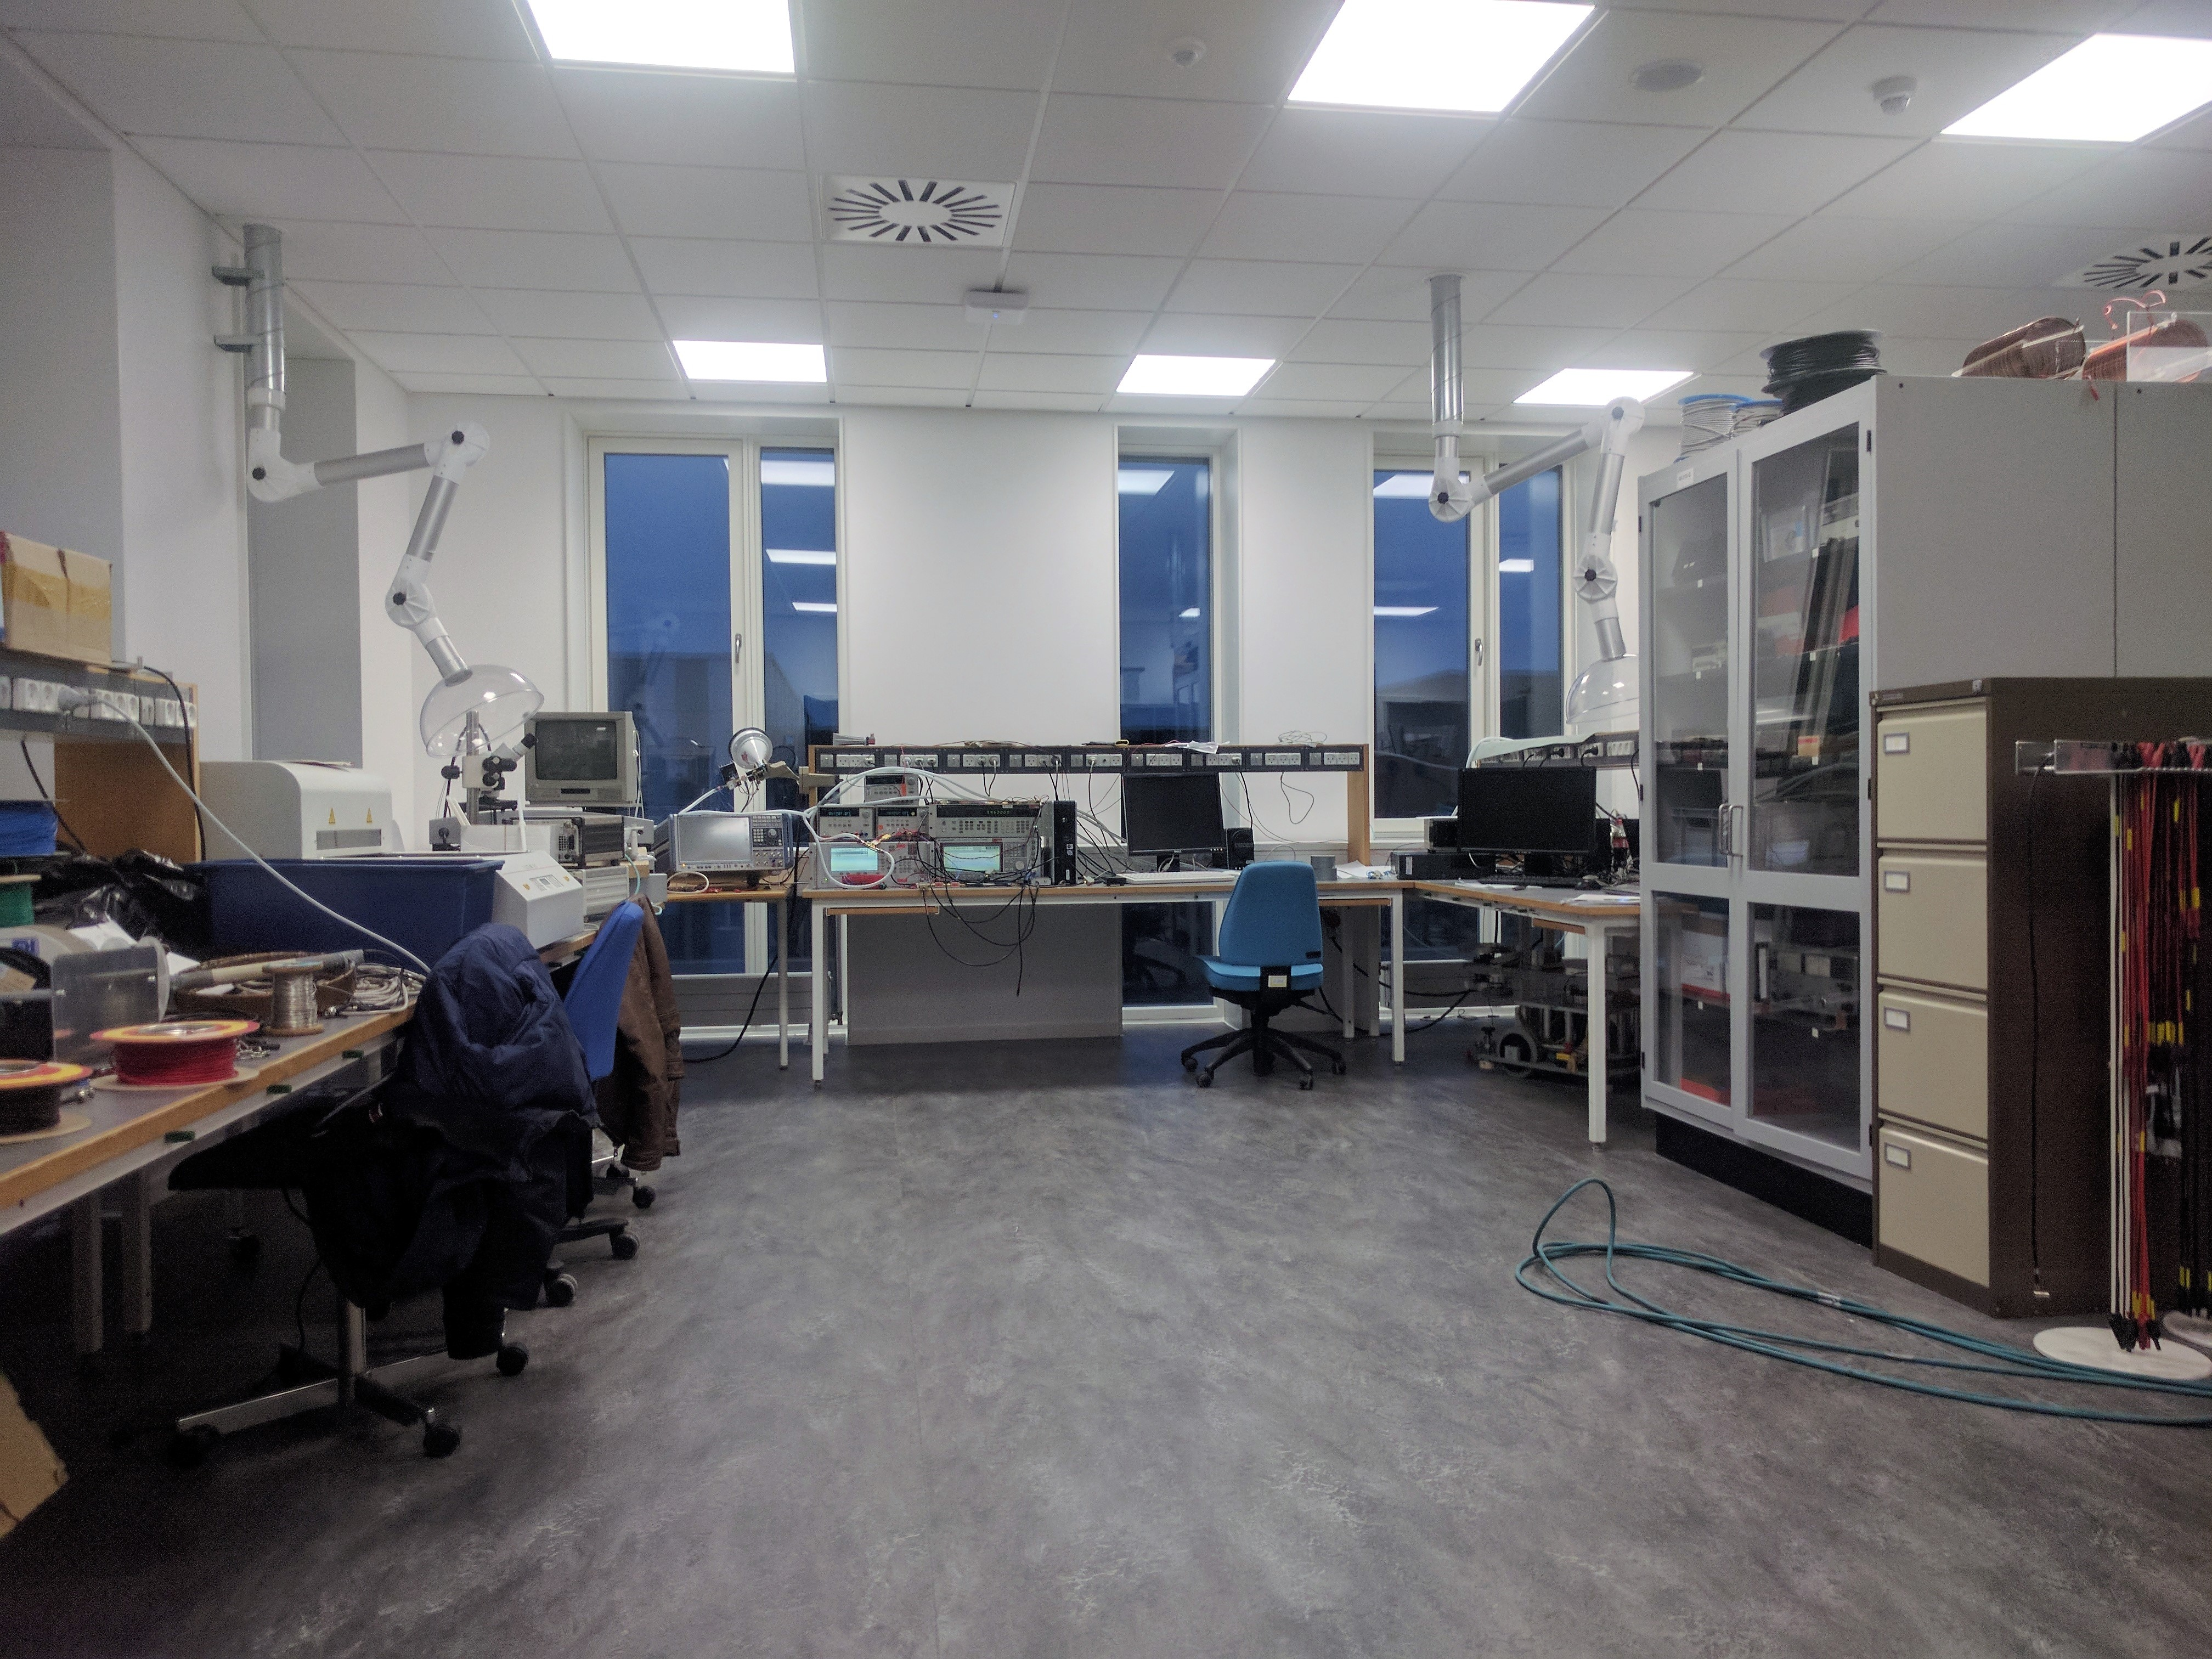
\includegraphics[width=\textwidth]{pictures/Measurement/walking_meas.jpg}
    \caption{Room overview with antenna placement}
  \end{minipage}
\end{figure}
\subsection{Fireplan}

%The setup of the measurement will give the insight and solutions to the problems hypothesised in previous chapters. 
%
%\begin{figure}[H]
%\centering
%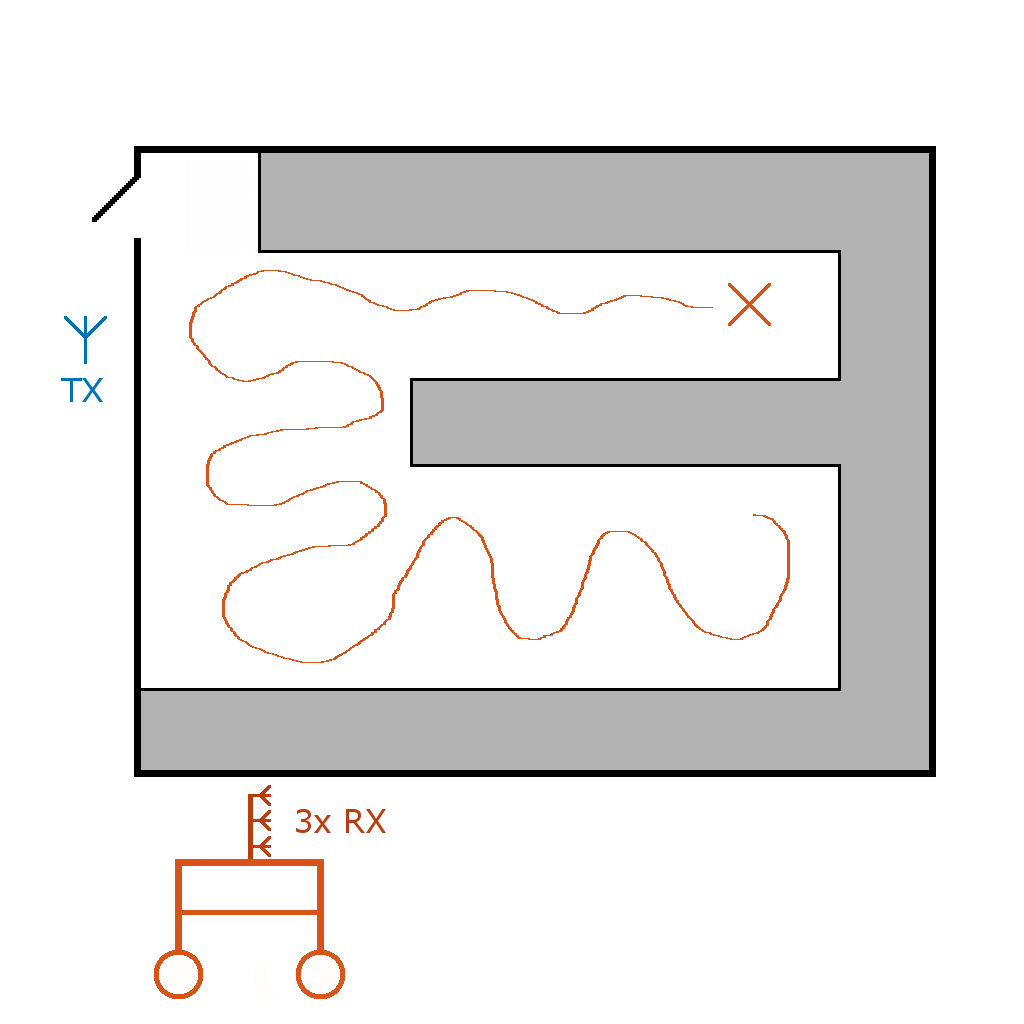
\includegraphics[width=0.75\textwidth]{figures/Gimp_figures/MeasSetup.png}
%\caption{Sketch of the room}
%\label{room sketch}
%\end{figure}
%
%The idea is to do a pilot test of the room. This is to obtain the pathloss $L$ and the delay spread of the room $\sigma_\tau$. With these values we can find the coherence bandwidth $B_c$ and the fading gain can be calculated. 
%We suspect that since this is a multipath NLOS setup the delay spread and pathloss will be very similar across the room. But as a precaution the rooms pathloss and delay will be measured in a close,mid and far region from the doors where the signal originates. When the measurements are ongoing there will be some loss associated with body loss of the handsome scientist and clutter in the environment. This will give more multipath reflections compared to a a empty room.
%\todo {read and rewrite to proper English}
%
%With the pilot test done the full measurement can begin. This will use the same setup as for the pilot test, but with three reviver antennas measuring in parallel and different settings on the VNA. Given the results of the pilot test the amount of samples the sweep will obtain in frequency $N_f$ can be terminated. With this the amount of samples in space can be found to get a total of $4.04 \cdot 10^6$ samples. when the measurement starts the antenna array will be moved slowly in space. During the measurement the operate of the PNA will indicate how fast the person holding the antenna array should walk.



\section{Equipment}
Keysight PNA N5527A 4-port VNA with parallel measurements and supports a frequencies from 10MHz to 67 GHz. With a 4 port VNA a antenna setup in a 1 TX and 3 RX configuration will be used. Calibration can be done by connecting the cables together and do a simple normalization. The sweep data will be saved to a USB.


Cables used have a loss of $0.5dB  \ per \ m$. 3 10m cables and 1 4m cable for the RX and TX antennas respectively. This gives a total cable loss $L_c$ of 7dB.

The TX antenna is a directional antenna with a gain of 12dBi at 5GHz.\todo {antenna gain appendix}
The RX antenna array is a omnidirectional antenna with a 5Ghz $f_c$ and a spacing of $>0.4 \lambda$.
\begin{figure}[H]
\centering
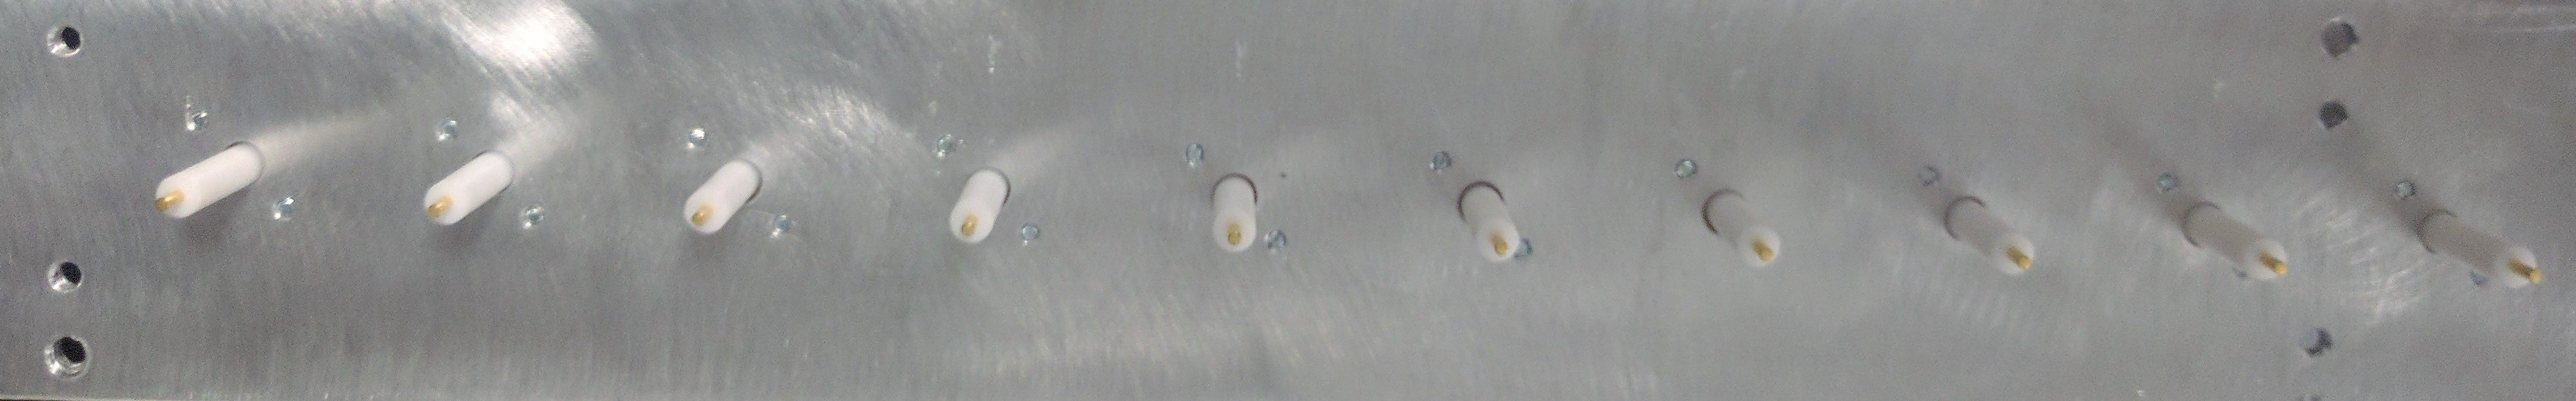
\includegraphics[width=0.7\textwidth]{pictures/Measurement/antenna_array.jpg}
    \caption{Omnidirectional RX antenna array with $\frac{\lambda}{2}$ spacing}
\end{figure}
\todo{add a schematic overview of the room}
\begin{figure}[H]
\centering
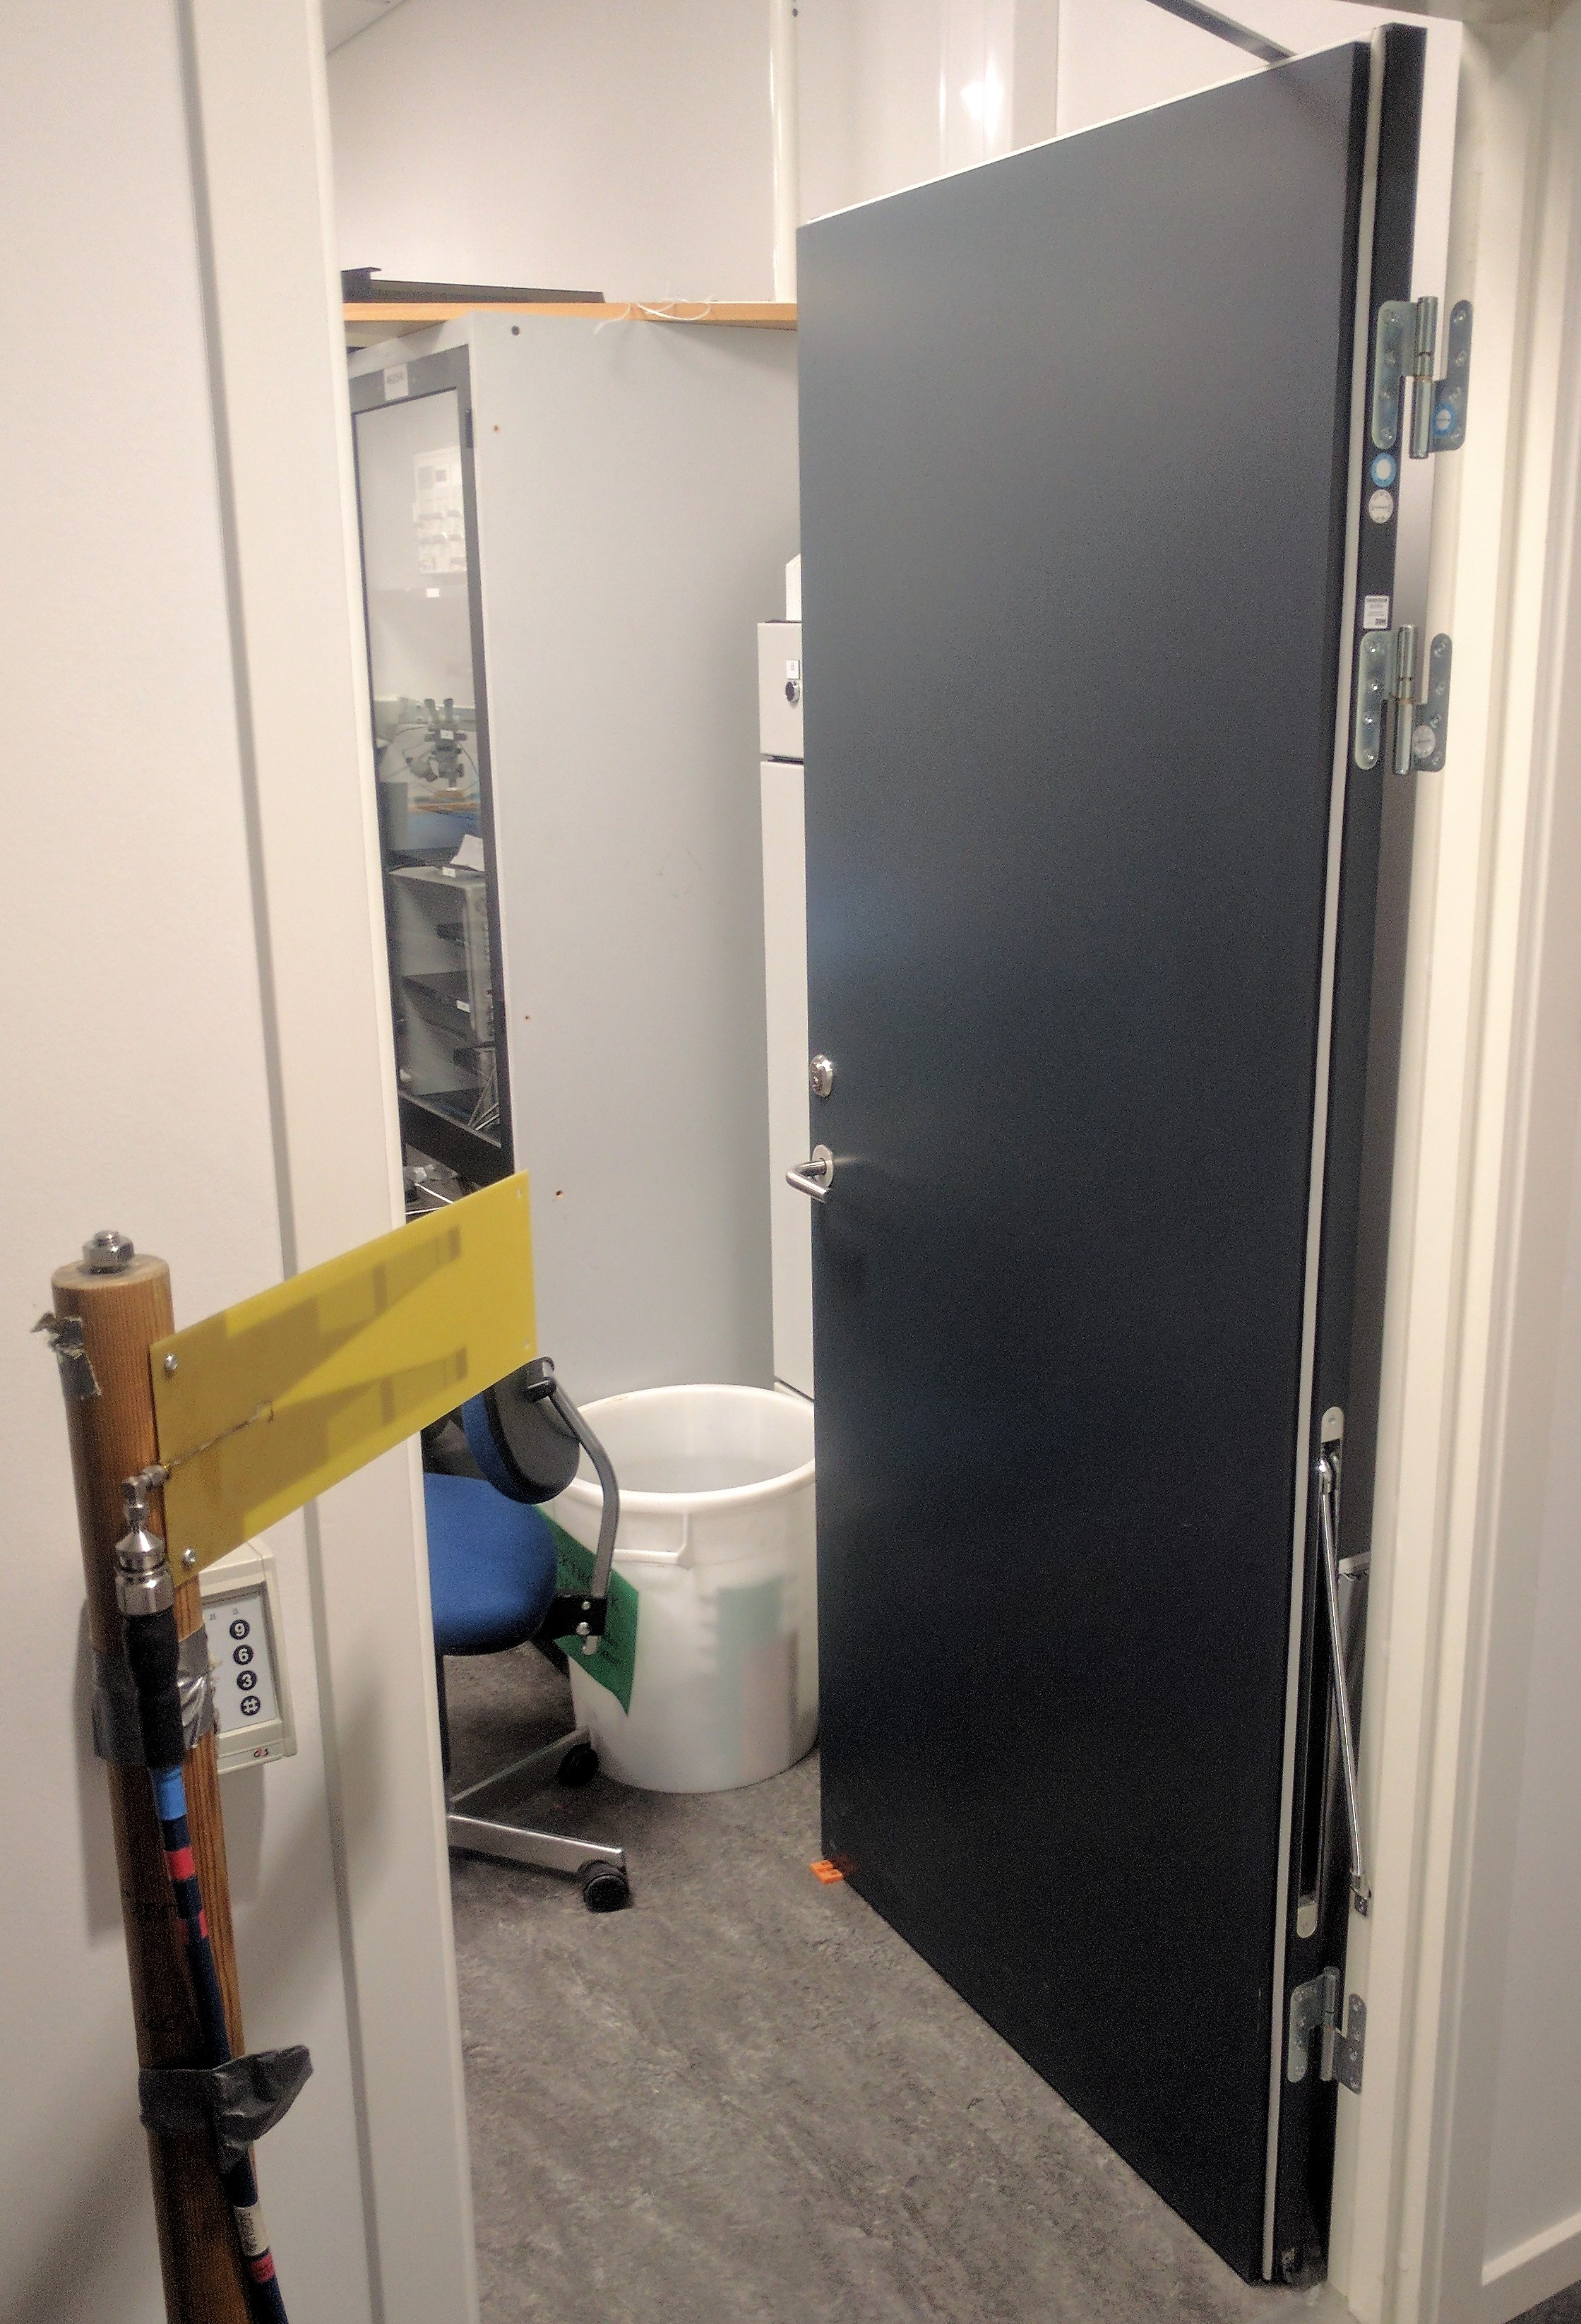
\includegraphics[width=0.4\textwidth]{pictures/Measurement/antenna_door.jpg}
\caption{Directional TX antenna pointing at door.}
\end{figure}


\label{equip}
\subsection{Connected setup}

\begin{figure}[H]
\centering
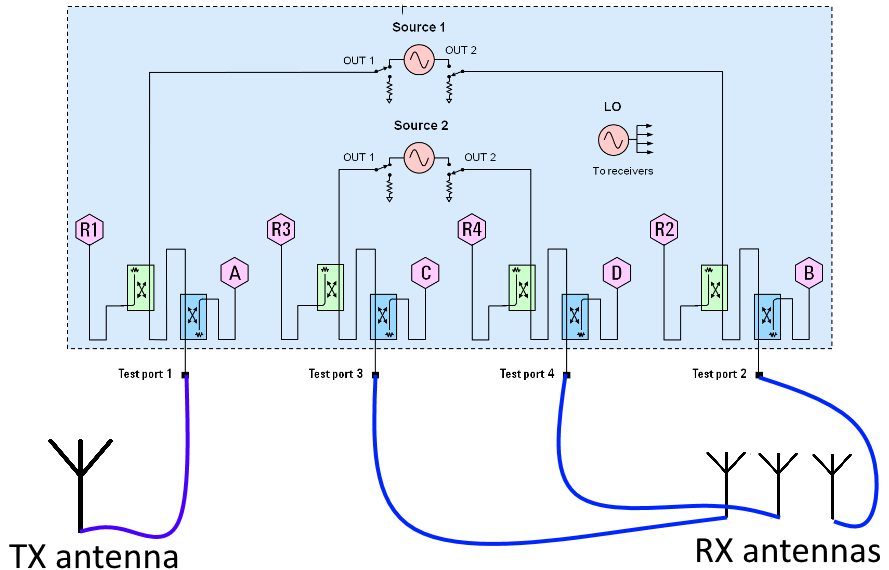
\includegraphics[width=0.65\textwidth]{figures/Gimp_figures/4portVNA.png}
\caption{VNA connections}
\label{connection_diagram}
\end{figure}

%Keysight PNA N5527A 4-port VNA with parallel measurements and supports a frequencies from 10MHz to 67 GHz. The sweep data will me saved to a USB.
%
%Cables used have a loss of $0.5dB per m$ 
%Splitter to separate the signal to two TX antennas and point towards the doors for more equal distribution of signal.
%N5527A has a $-119dB$ noise floor without averaging with a 10Hz $IF_{bw}$ at 1-10GHz. The dynamic range of the VNA becomes:
%
%\begin{equation}
%DR = P_{tx}-119dBm 
%\label{NFvna}
%\end{equation}


\section{Final setup}
After playing around with the test setup we discovered that to reduce the pathloss and cable loss the directonal TX atenna was moved closer to the door. Still NLOS was true as the antenna was outside of the room pointing at a open door.





%The most important part of the setup is the equipment and how they are connected. The R\&S Spectrum Analyser (model FPL9KHz-6GHz) is the center of the setup. This is the receiver of our system and gives us a readout of the spectrum in terms of power (dBm) and frequency (Hz). The two main setting on the Spectrum analyser is IF filter bandwidth and resolution. These two values gives us a sweep time.
\chapter{Setup Parameter estimation}
In chapter 1 all the needed factors has been discussed. The parameter of the test setup and the requirements where:

\section{Dynamic range}
N5527A has a $-119dB$ noise floor without averaging with a 10Hz $IF_{BW}$ at 1-10GHz\autoref{equip}. The dynamic range of the VNA becomes:
\begin{equation}
DR = P_{RX}+119dBm 
\label{NFvna}
\end{equation}

\subsection{TX power}
The transmit power $P_{TX}$ is the maximum power the VNA can transmit without getting overloaded. This should be around 15dBm\autoref{equip} depending on load from the different antennas.
\subsection{Pathloss}
Given \autoref{eq:path_loss} and the area of the room. The planned walking route in the room is around 6 meters from the antenna. This gives a pathloss value of:
\begin{equation}
L = 20log (5000) + 28 \cdot log(6)-28 = 67.76dB \approx 68dB
\label{eq:path_loss}
\end{equation}

The $P_{RX}$ becomes:
\begin{equation}
P_{RX} = 15dBm + 12dBi - 68dB = -41dBm
\end{equation}
This gives a maximum dynamic range of:
\begin{equation}
DR = -41dBm+119dBm = 78dB
\end{equation}


\subsection{IF-bandwidth(noise floor)}
Given the SNR margin $SNR_{M}$ and the $P_{RX}$ the noisefloor needs to be at:
\begin{equation}
Noisefloor_{Req} = -41dBm-64dB = -105dBm 
\end{equation}
The noise floor of the \gls{VNA} scales linearly with a increased $IF_{BW}$\citep{PNA_scale}. This would mean that a $IF_{BW}$ on the \gls{VNA} can be increased by:
\begin{equation}
\begin{split}
&= IF_{BW} = -119dB+105dB = 14dB \\
          \quad &= 10Hz \rightarrow 14dB \rightarrow 250Hz
\end{split}
\end{equation}
This means the $IF_{BW}$ can be at 250Hz, this will give us faster sweep times at the cost of dynamic range.
\section{FCF}
This section needs some values from similar environments 50-150ns delay.
\section{Time estimation}
Since the \gls{VNA} can do segmented sweeps the sweep time is mostly dependant on the number of points and $IF_BW$.
The Keysight PNA N5527A gives the following sweep times for a 201 point with different $IF_{BW}$ \citep{Key_PNA}.

\begin{table}[H]
\centering
\caption{$IF_{BW} \ vs \ sweep time$}
\label{my-label}
\begin{tabular}{l|l}
\hline
$IF_BW${[}Hz{]} & Sweep time {[}ms{]} \\
10              & 17834               \\
100             & 1825                \\
300             & 641                 \\
1000            & 223                 \\
3000            & 72                 
\end{tabular}
\end{table}

There is also some overhead for saving the data. Since number of points used in the final setup is dependant $B_c$ the sweep time 

Let's use example where we can use a 1kHz $IF_BW$ a
\begin{equation}
T_{sweep total} = 223ms
\end{equation}
This means that every 223ms we have to move $\frac{\lambda}{2}$ this gives a relative velocity of:
\begin{equation}
\frac{0.0375m}{0.223s} = 0.17 m/s
\end{equation}
This is under the $1m/s$ value found in \autoref{min_vel}
and total time for moving 5 meters $\approx 30s$.
and with the speculated 80000 samples per 5 meter walk(200 samples in frequency). we need around:
\begin{equation}
\frac{4.04 \cdot 10^6}{80000} = 50.5 walks
\end{equation}
or around 25 minuets of measurement given 55.5 walks and 30s per walk and no wait time.

\chapter{Measurement of PDP}
\section{setup}
\section{results}
\section{data processing}
\subsection{delay spread}
\subsection{coherence bandwidth}

\chapter{Measurement of fading}
\begin{table}[H]
\centering
\caption{Some example specifications}
\label{final_specs}
\begin{tabular}{|l|l|l|}
\hline
Number of samples needed         & N           & 4.04 million         \\ \hline
Center Frequency                 & $f_c$       & 5Ghz             \\ \hline
Wavelength                       & $\lambda$   & 6cm           \\ \hline
Coherence freq                   & $\Delta f$  & 25MHz           \\ \hline
Span & $\delta f$ & 1GH \\ \hline
Dynamic range                    & DR          & XXdB            \\ \hline
Antenna diversity                & $A_{div}$   & 1x3                    \\ \hline
Intermediate frequency bandwidth & $IF_{BW}$     & 500Hz          \\ \hline
Number of points per sweep & $N_{sweep}$ & 41 \\ \hline
Transmit power & $P_{TX}$ & 17dBm \\ \hline
Sweep time & $T_{sweep}$ &74.1msec \\ \hline
\end{tabular}
\end{table}
These where the final values used in the VNA to do the measurements.
\section{setup}
\section{results}
\section{data processing}
\subsection{stationarity}
K-factor
\subsection{achieved dynamic range}
\subsection{frequency correlation}
\subsection{space correlation}
\subsection{approximate N equivalent}
\subsection{CDF}
confidence values - bootstrap

\section{Results}